\documentclass[a4paper]{article}
\usepackage[T1]{fontenc}
\usepackage[utf8]{inputenc}
\usepackage{mlmodern}
\usepackage{graphicx}
\usepackage{geometry}
\usepackage{float}
\geometry{a4paper, top=15mm}
\usepackage[parfill]{parskip}
\usepackage[colorlinks=true,naturalnames=true,plainpages=false,pdfpagelabels=true]{hyperref}

\usepackage[backend=biber, sorting=none]{biblatex}
\addbibresource{uni.bib}

\usepackage{amssymb}
\usepackage{amsthm}
\usepackage{mathtools}



\title{University of Vienna\\
\vspace{1cm}Seminar:\\Complex Network Analysis\\
\vspace{0.5cm}Python Package-Dependency Network
}
\author{Milutin Popović}

\begin{document}
\maketitle

\section{Introduction}

The following project will map python packages and their dependencies into a
time dependent directed graph(complex network), analyze the graph and
visualize it Virtual-Reality (VR). Most python packages have a given set of
dependencies that are needed to use the specific package. Both the package
and the dependency will represent a vertex. The directional edges between
packages will represent their dependence. Note that it is also possible for a
package to have no dependency, in this case it will have no outgoing edges
and the construction of the graph will avoid self loops for such specific
cases. The main analysis of the graph will evolve around the growth exponent
of nodes. Based on the covariance of the fit of the cumulative logarithmic
growth function. The analysis will separate the best performing
packages(nodes) released not before 2016.

\section{Data}
At the time of this doing this project the number of nodes was around
$3.6\cdot10^{5}$ and the number of links was around $10^{6}$. The data is
sourced from the Python Package Index(PYPI) main website \cite{pypi}. The
gathering of the data resorts to first of all finding out the names of all
the packages then with this information browse the \textit{json}-quivery of
PYPI for every package. The provided data by the Python Package Index has a
\textit{json} type structure for all packages, which includes both the
release date and the dependencies of a specific package(and a lot of other
information too).


Querying through all packages
and writing an edge-list in the package-dependency format gives a directed
network as is.

The important thing is that, given the release information for each package
the graph can be restructured by time steps from the time the first package
was released to the time the last package was released. The reconstruction
will create a network for each month from around the start of the year 2005
to the middle of the year 2022. The edge-list as described above together
with the time stamps of the package releases will be treated as a single data
entry, even though it is not because the edge list represents a connection
between a package and its dependency while the release date is only of the
package and not not its dependency. The first sorting will create a file for
the package) inside the file. The second sorting will go through all of the
files(months) again and check if the dependency of a package was indeed
released, if not it will buffer it and delete the connection to the package
in the current file. Later on when the actual dependency is released, only
then the deleted entry (package-repository) would be added from the buffer to
the currently selected file.

This turns out this is a sorting problem requiring a lot of buffer and
relying on loops, where python may not the best language for the task. That
said I would advise against executing this code since it needs to sort and
resort $10^{6}$ links based on their time stamp.

The data and code for sorting can be found under my Github instance
\cite{sorting}.

\section{Implementation and Analysis}
The implementation of the whole project can be found under my Github instance
\cite{impl}.

To first of all build a general understanding of then network, a simple
degree distribution observation of the last time step (current day network)
was made. As most complex networks in the internet, this network also follows
a power law distribution. In the figure bellow the degree distribution is
show for the network, without incorporating directionality of the network.
\begin{figure}[H]
    \centering
    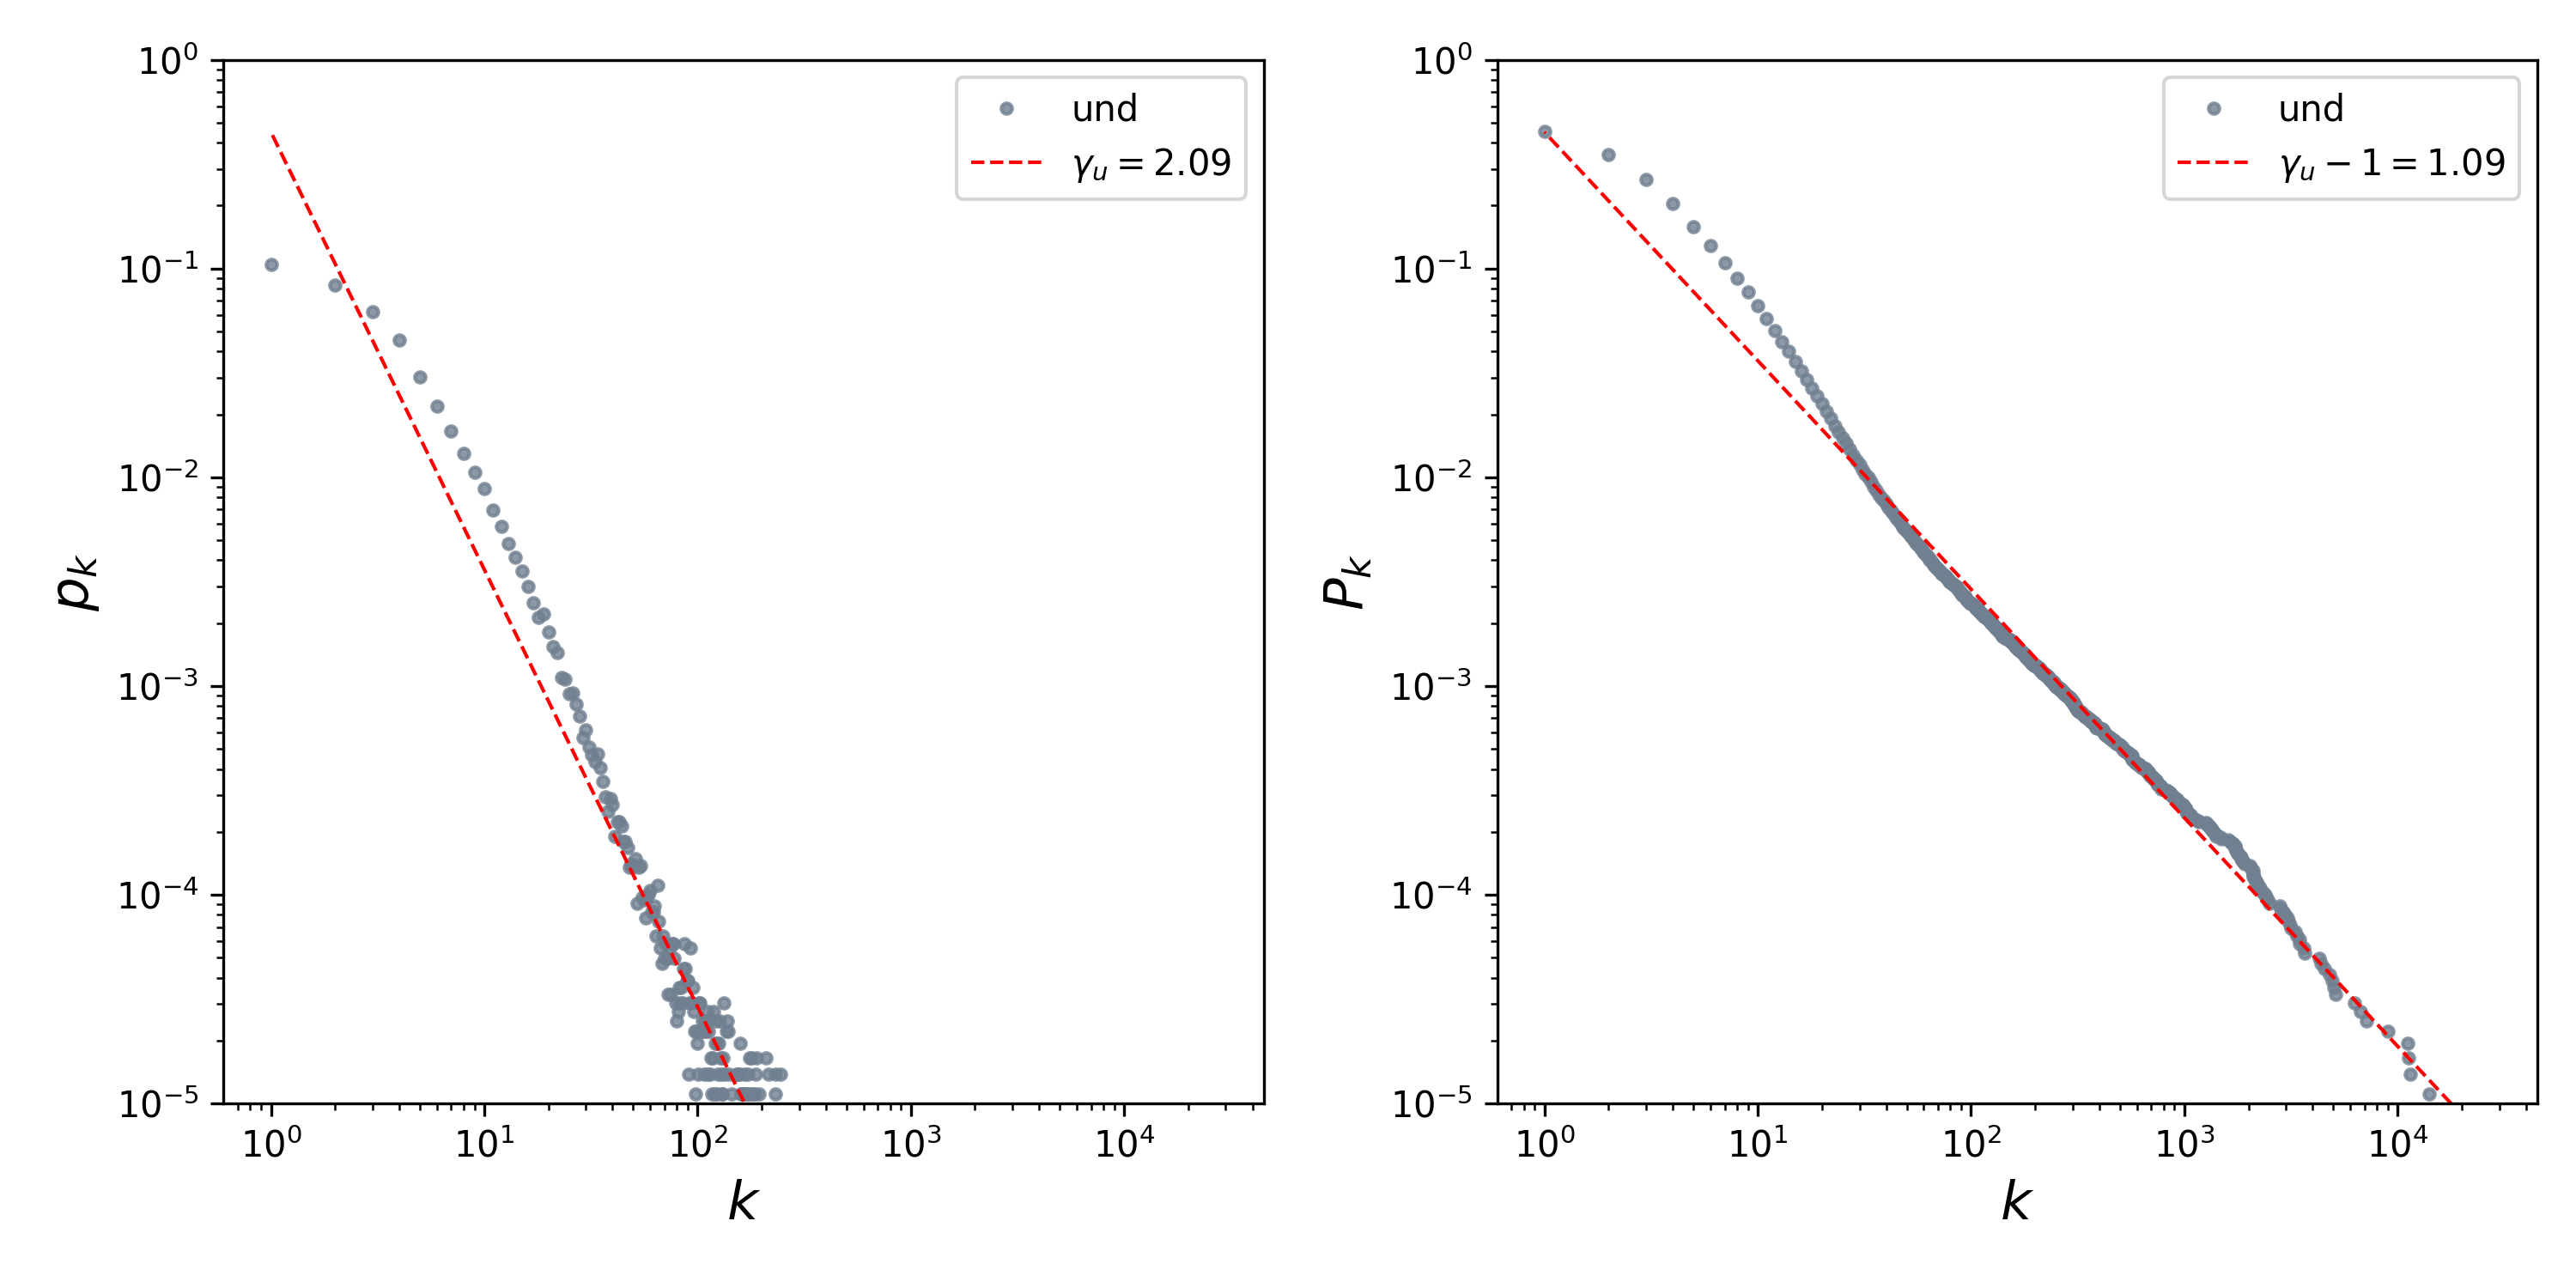
\includegraphics[width=0.8\textwidth]{../pres/pics/dist_u.png}
    \caption{The left picture shows the power law distribution, the right
    the cumulative degree distribution, both in log-log scales and both
    without incorporating directionality. The red dotted line is the regression fit}
    \label{dist_u}
\end{figure}
The second case differentiates between outgoing links and incoming links,
the observations are rather similar
\begin{figure}[H]
    \centering
    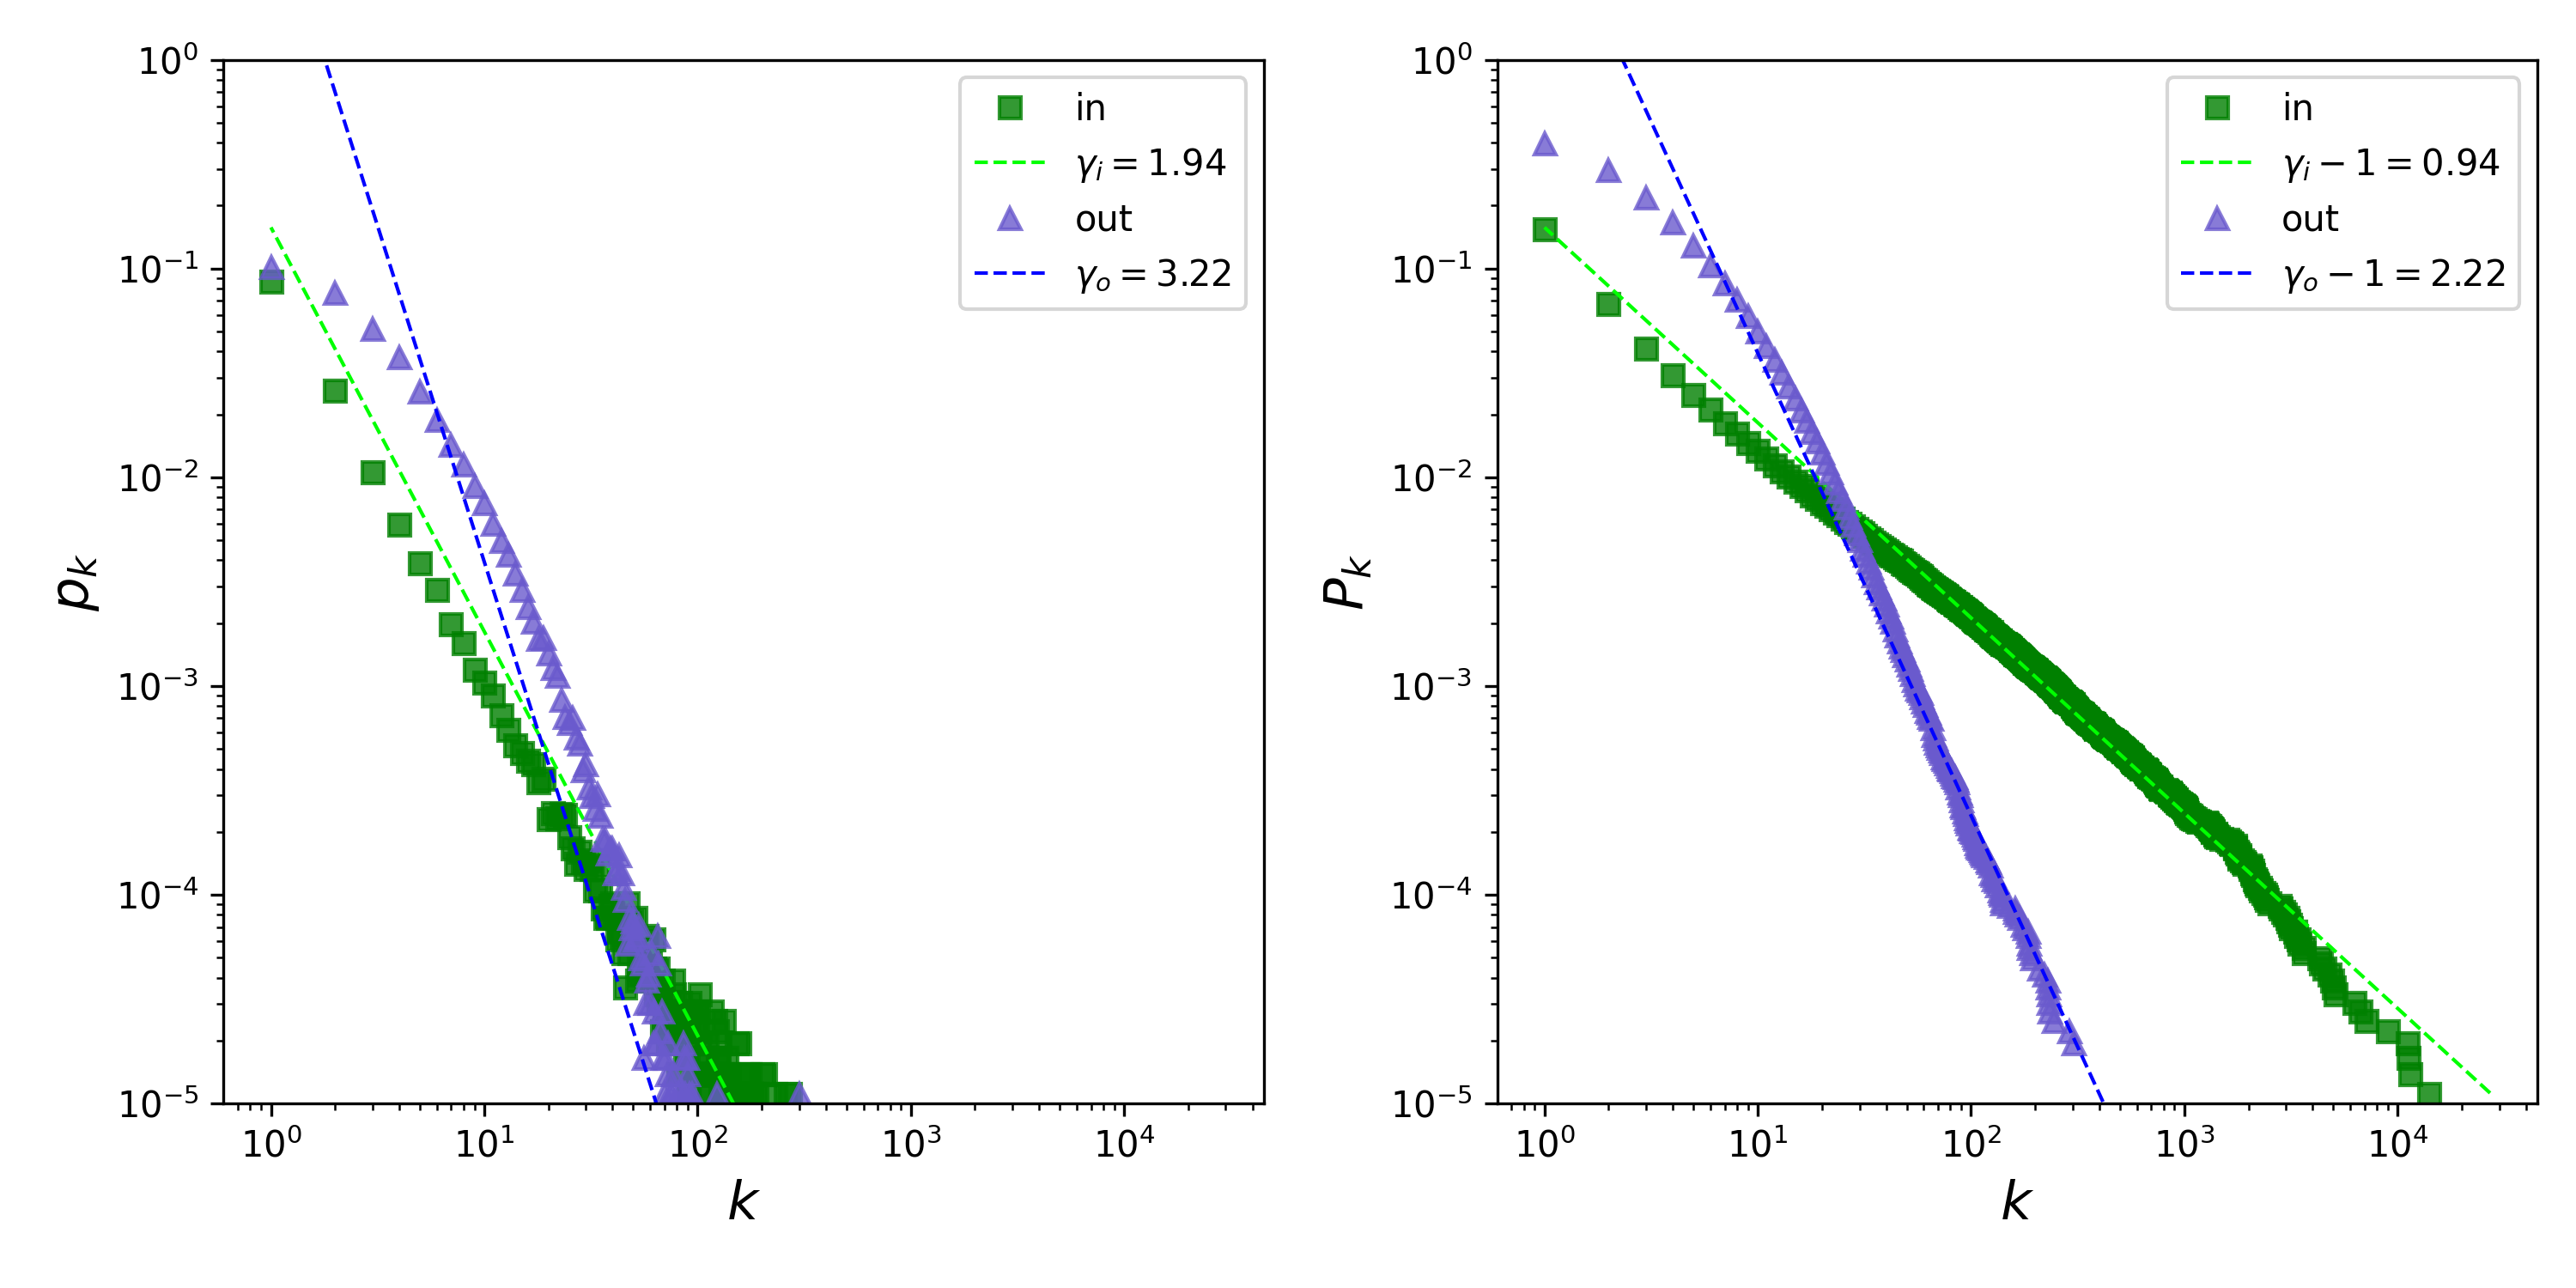
\includegraphics[width=0.8\textwidth]{../pres/pics/dist_d.png}
    \caption{The left picture shows the power law distribution of in-degree
        represented by green squares, out-degree represented by blue
        triangles. The right picture shows the cumulative degree
        distribution, both in log-log scales. The blue and green dotted lines are
        regression lines of in and out degree respectively}
    \label{dist_u}
\end{figure}
Another rather interesting thing, is to look at how well different nodes are
ranked in the network based on centrality measures. The figure bellow shows
such analysis.
\begin{figure}[H]
    \centering
    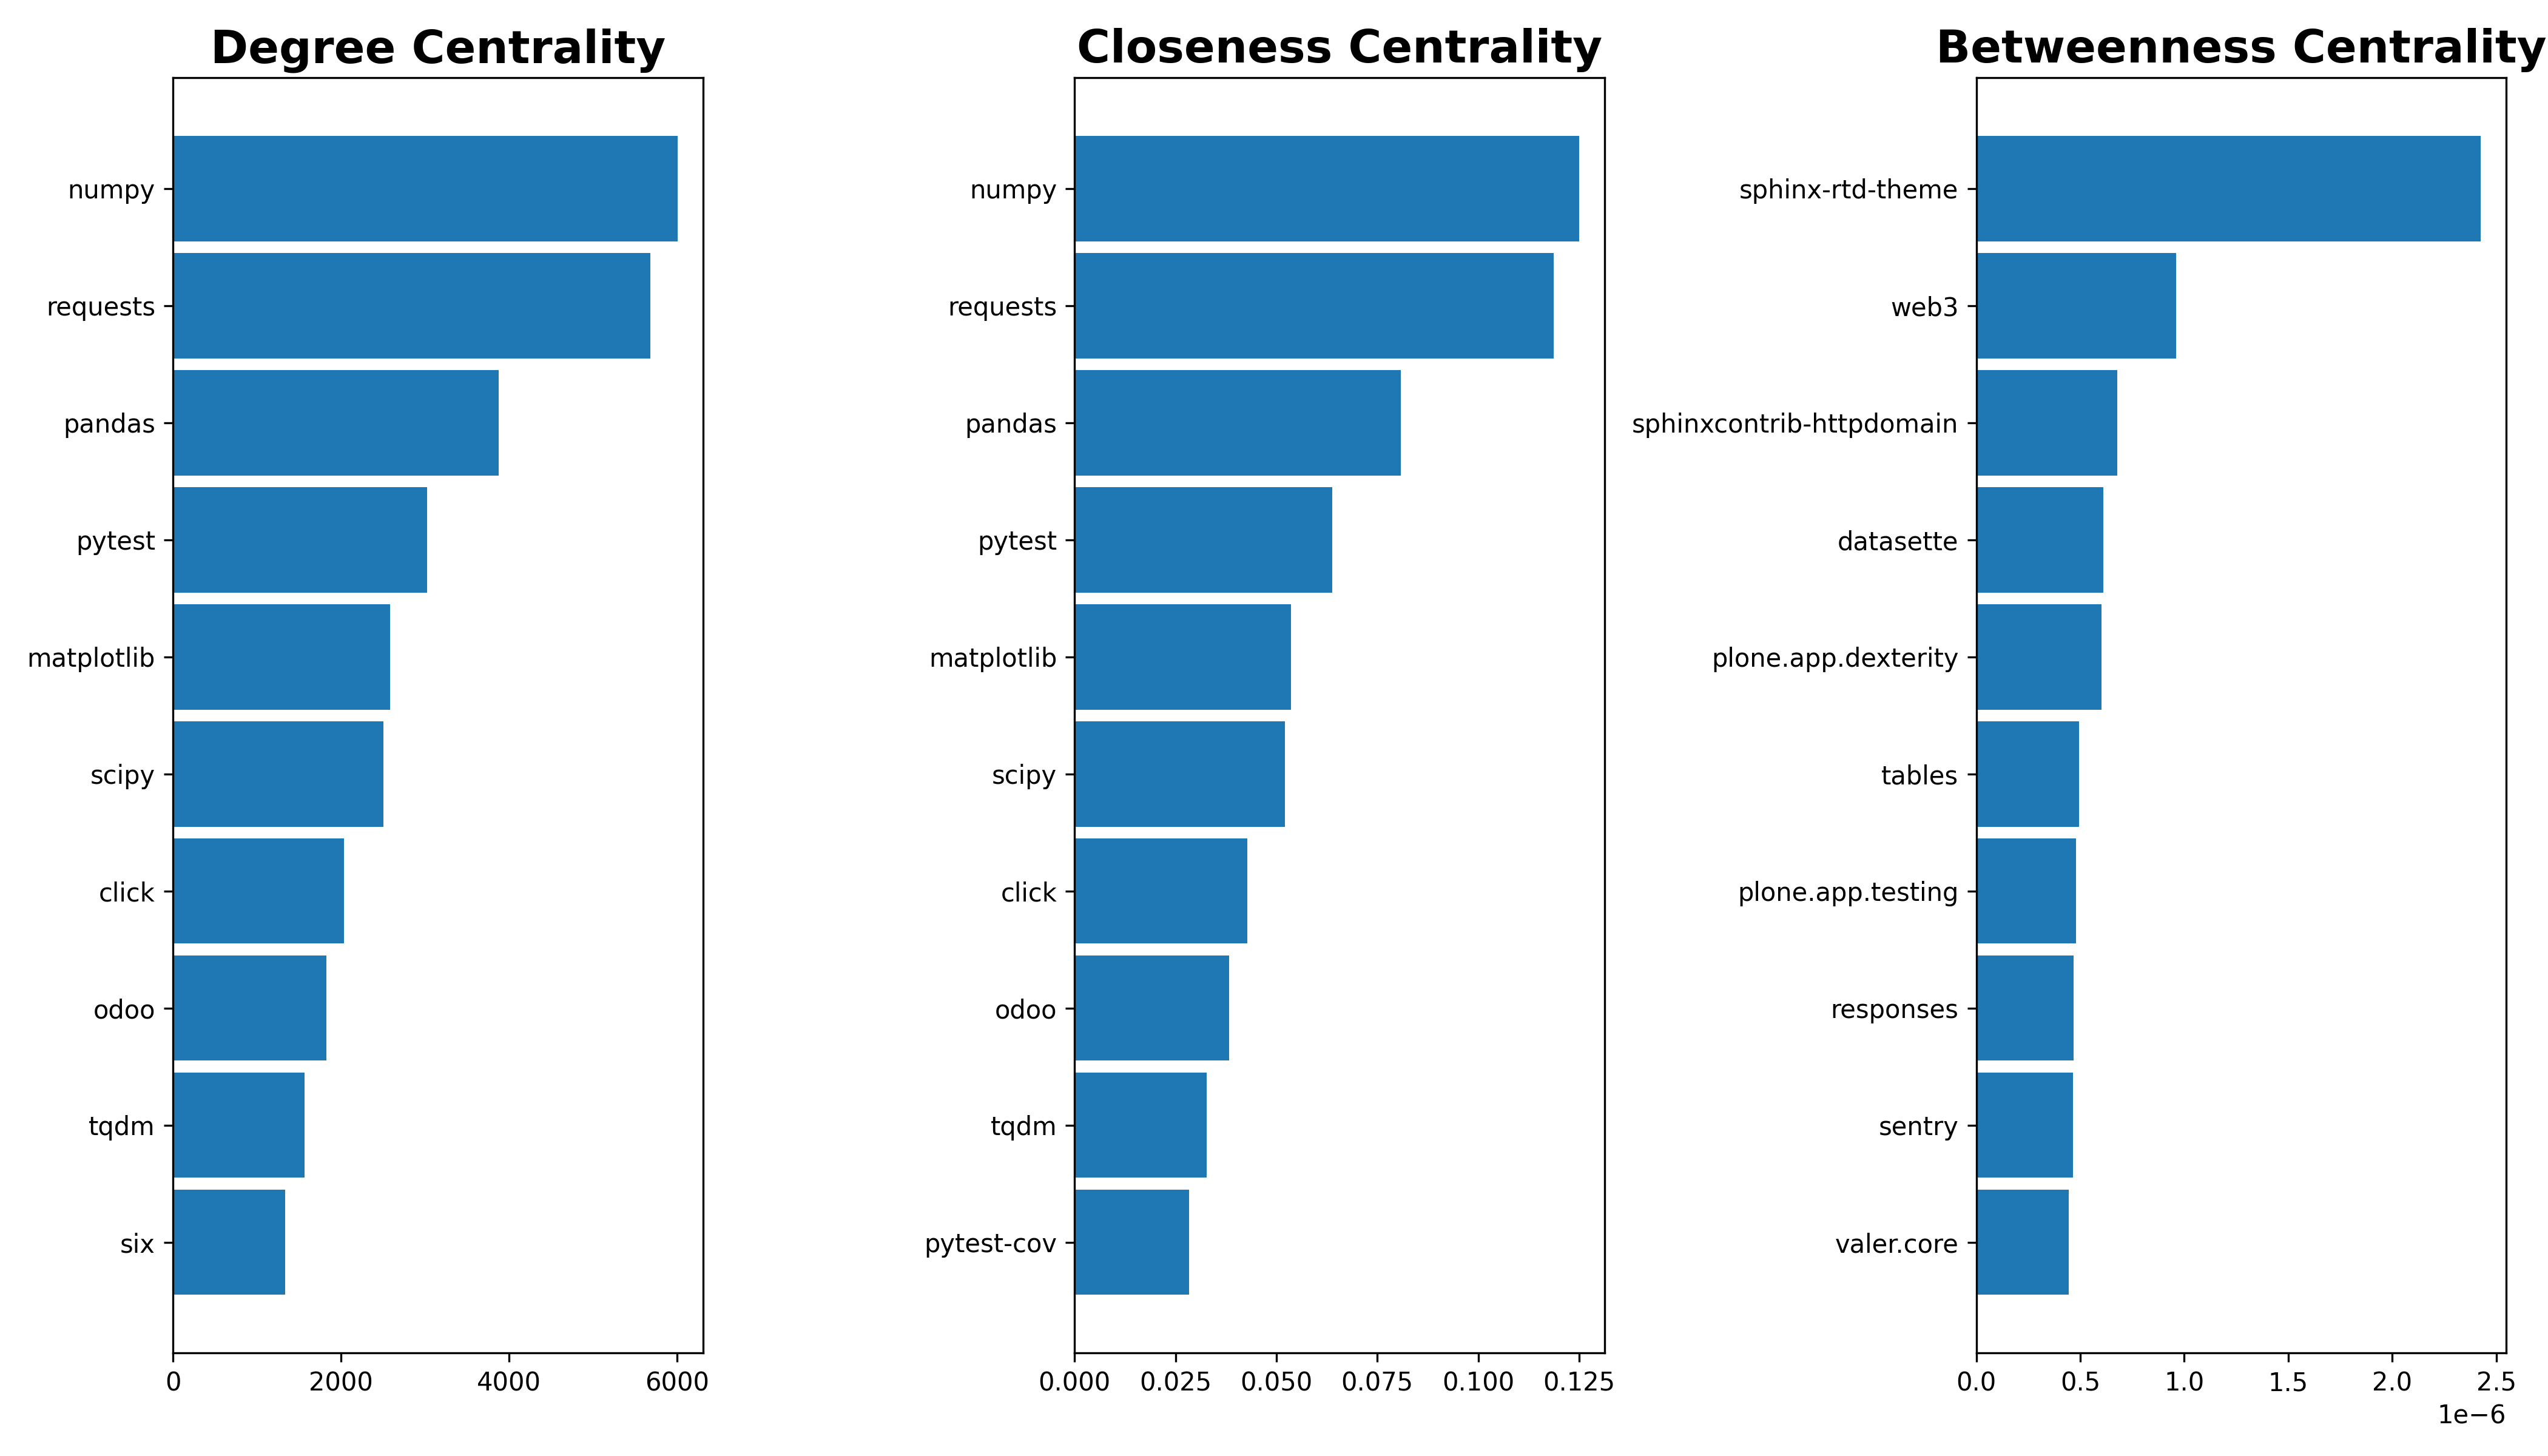
\includegraphics[width=1\textwidth]{../pres/pics/sneak_peak.png}
    \caption{Centrality measures of the network}
\end{figure}

As for the analysis of the time evolving network, the given tools by the most
common network analysis python programs do not have a way of dealing with
such networks. That is why a child class of the class \texttt{nx.DiGraph} is
invented, calling it \texttt{TDiGraph}. The general concept of this class is
that it incorporates all the class methods of \texttt{nx.DiGraph} and adds an
additional input and three more methods. The additional input is a list of
tuples containing a time stamped edge list in the format \texttt{(package ->
dependency, at time $t$)}. This allows us to create first of all two methods,
starting with a graph at $t=T_i$ the method \texttt{forward} would add all
edges corresponding to time $t=T_{i+1}$ and label the network to be at time
$t=T_{i+1}$. The second method does exactly the reverse and removes nodes
labeling the network to the time $t=T_{i-1}$ this method is called
\texttt{backward}. The third method allows to instantly go to a specific time
from $t=T_k$ to $t=T_i$ for both $k<i$ and $i>k$, doing nothing at $i=k$.
Specifically the first two methods, \texttt{forward} and \texttt{backward}
allow for the iteration over the network. This is especially practical since at
each time step different analytical information is obtained. For example degree
growth over the months shown in the figure bellow.
\begin{figure}[H]
    \centering
    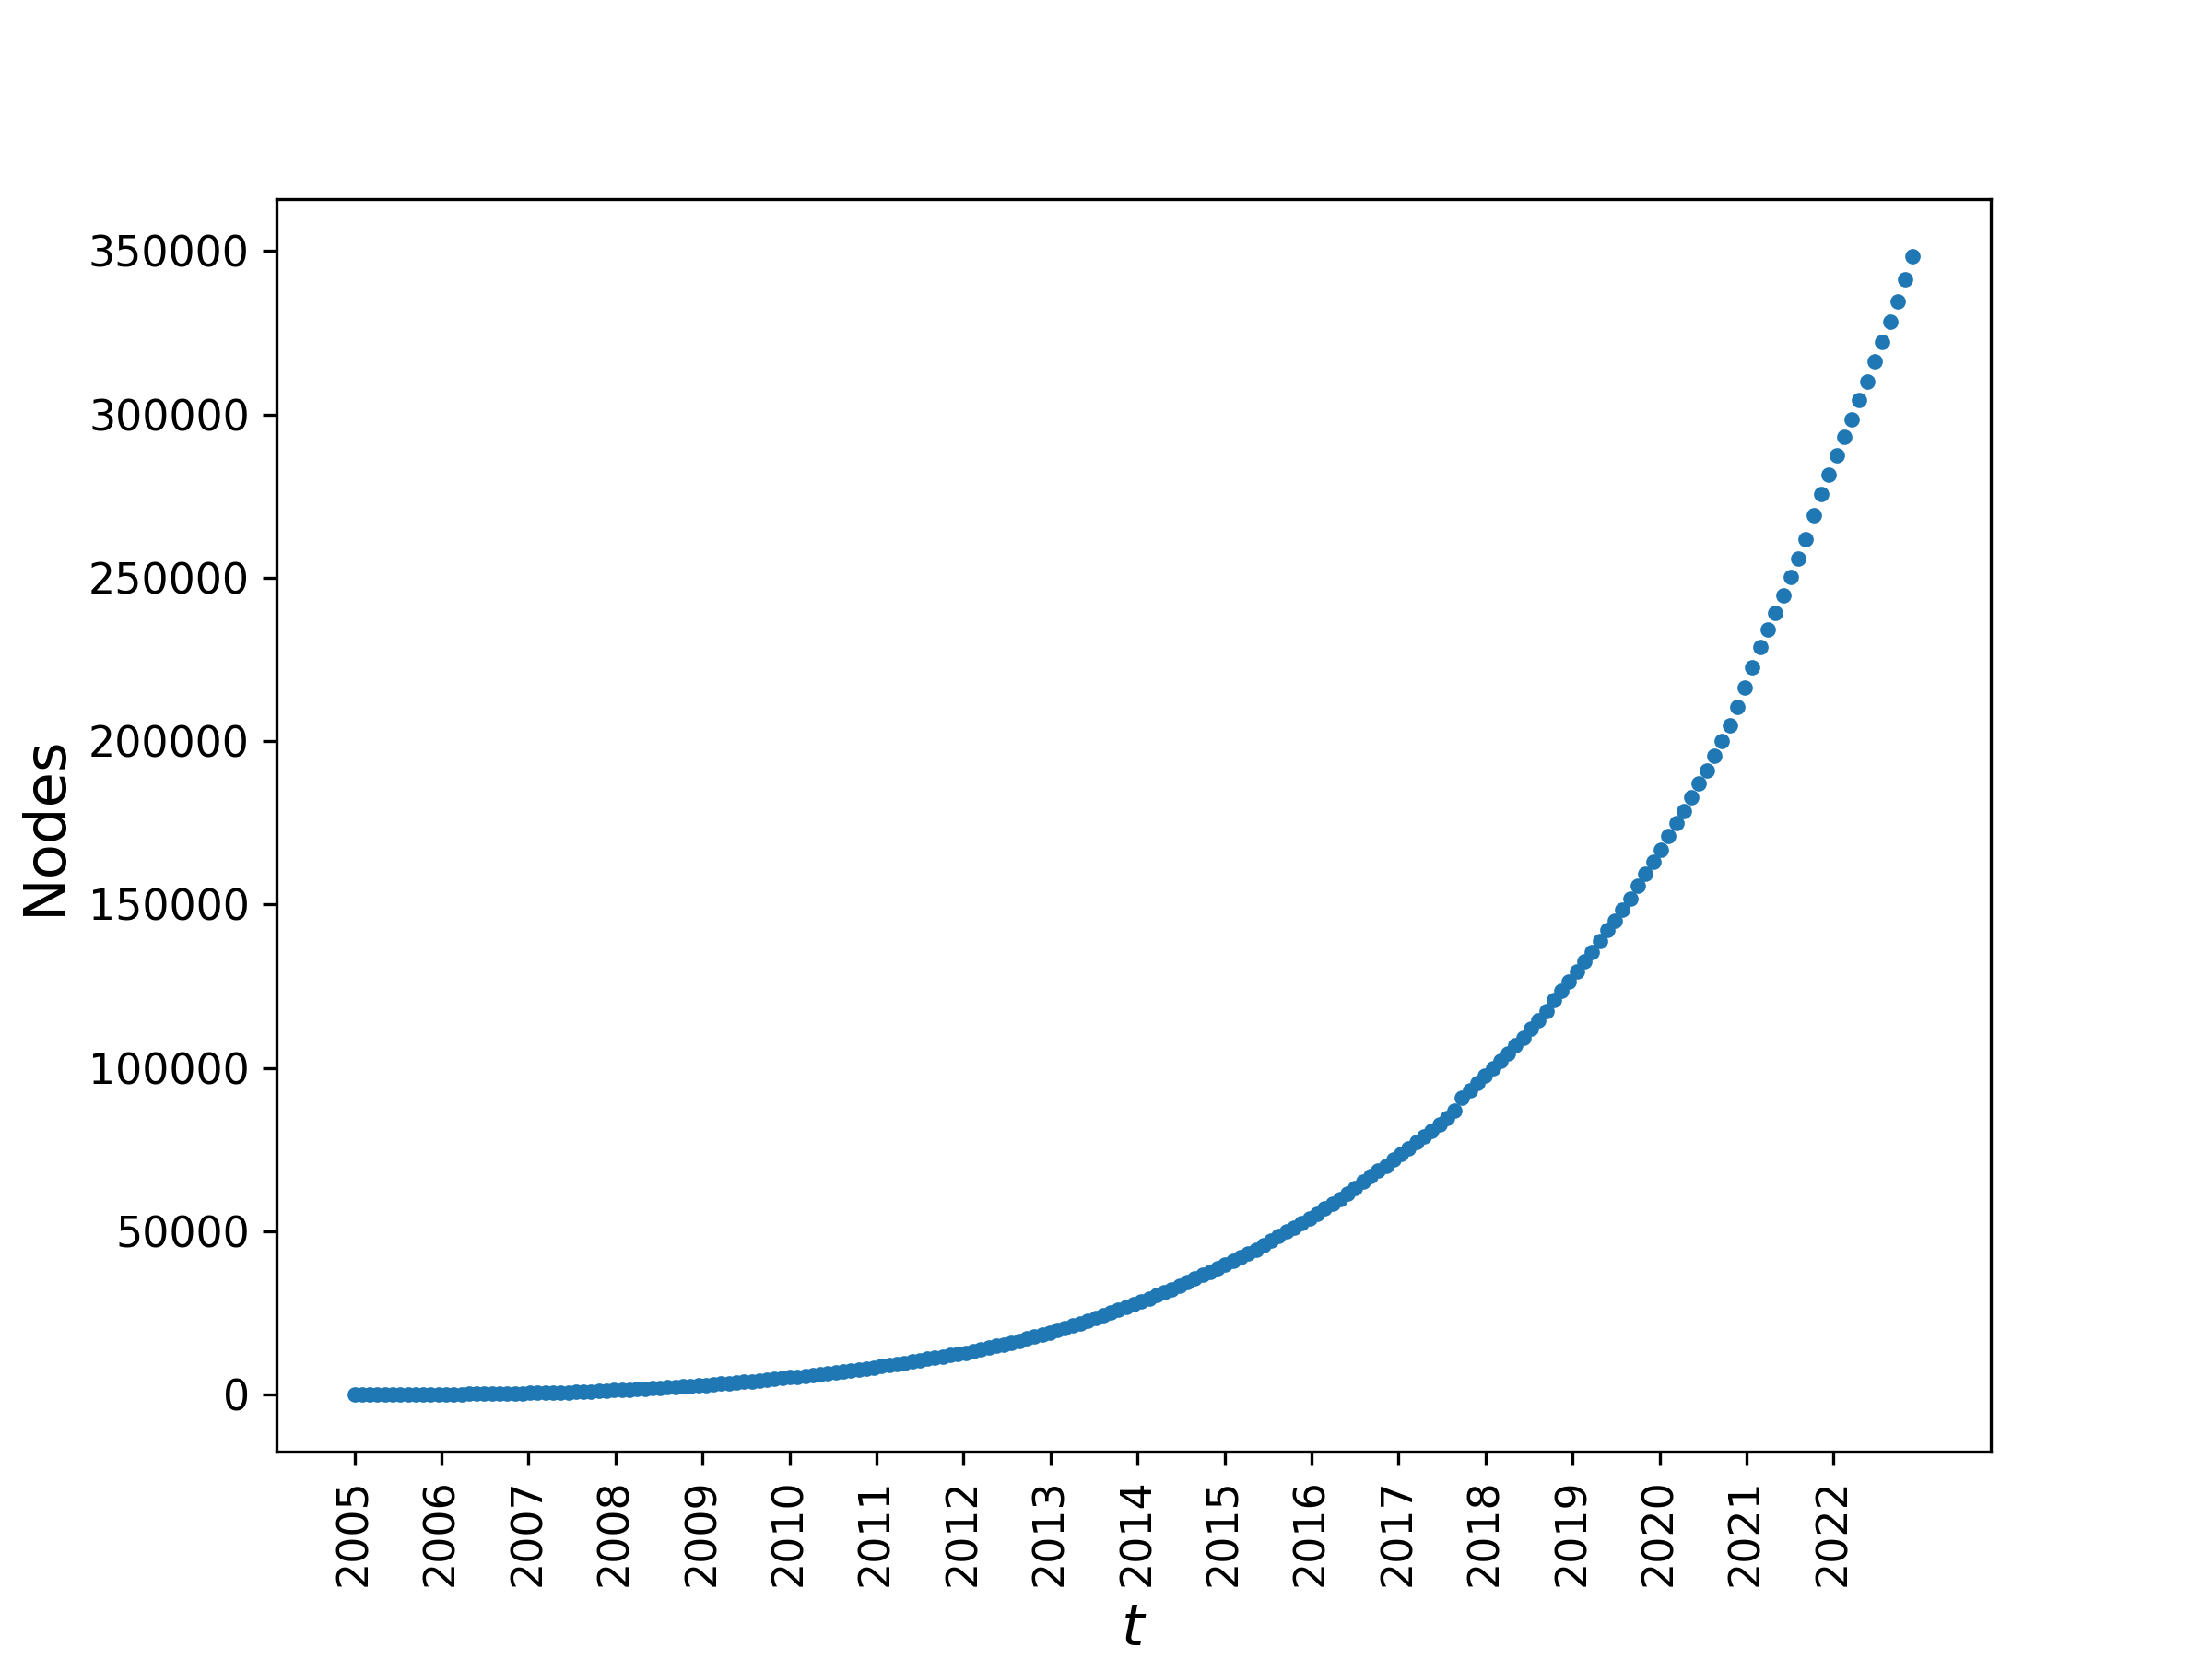
\includegraphics[width=0.8\textwidth]{../pres/pics/deg_growth.png}
    \caption{Node growth in the network over the months}
\end{figure}
Now that the basics are out of the way, a rather interesting prediction to
make is to separate python packages that have performed based on their
\textbf{in}-degree growth rather well and were created in the last couple of
years. The first problem encountered, is that the degree growth of a specific
node has a lot of noise, compared to theoretical models. To avoid this it is
more intuitive to consider the cumulative degree growth, in this case the
curve will be somewhat smoother. The second problem is that even thought this
is a scale free network there are all kinds of degree growths in this network
which do not coincide with theory in \cite{barabasi}. The theory fits a model $k_i(t) =
\left(t/t_i\right)^{\beta_i}$ of degree growth, as mentioned above
the analysis considers the cumulative degree growth and additionally will fit
in the standardized log scale. Then the function fit is linear $\beta_i \cdot x
+ c$ for given $x$. The main objective is to find all the $\beta_i$'s
corresponding to the nodes. Since there are all kind of degree growths, it is
worth only considering certain fits satisfying that $\text{CoV}(\beta)$ is
under a certainly well chosen threshold, then  a wide separation of nodes is
already established. It is also worth to motion here, that some test
statistic can be used such as the $\chi^2$ test. But when dealing with a
large number of fits, for the sake of computational cost only a $\text{CoV}$
threshold is considered. Together with considering only packages that were
released not before 2016 the following packages are given by the analysis,
shown in the figure below.
\begin{figure}[H]
    \centering
    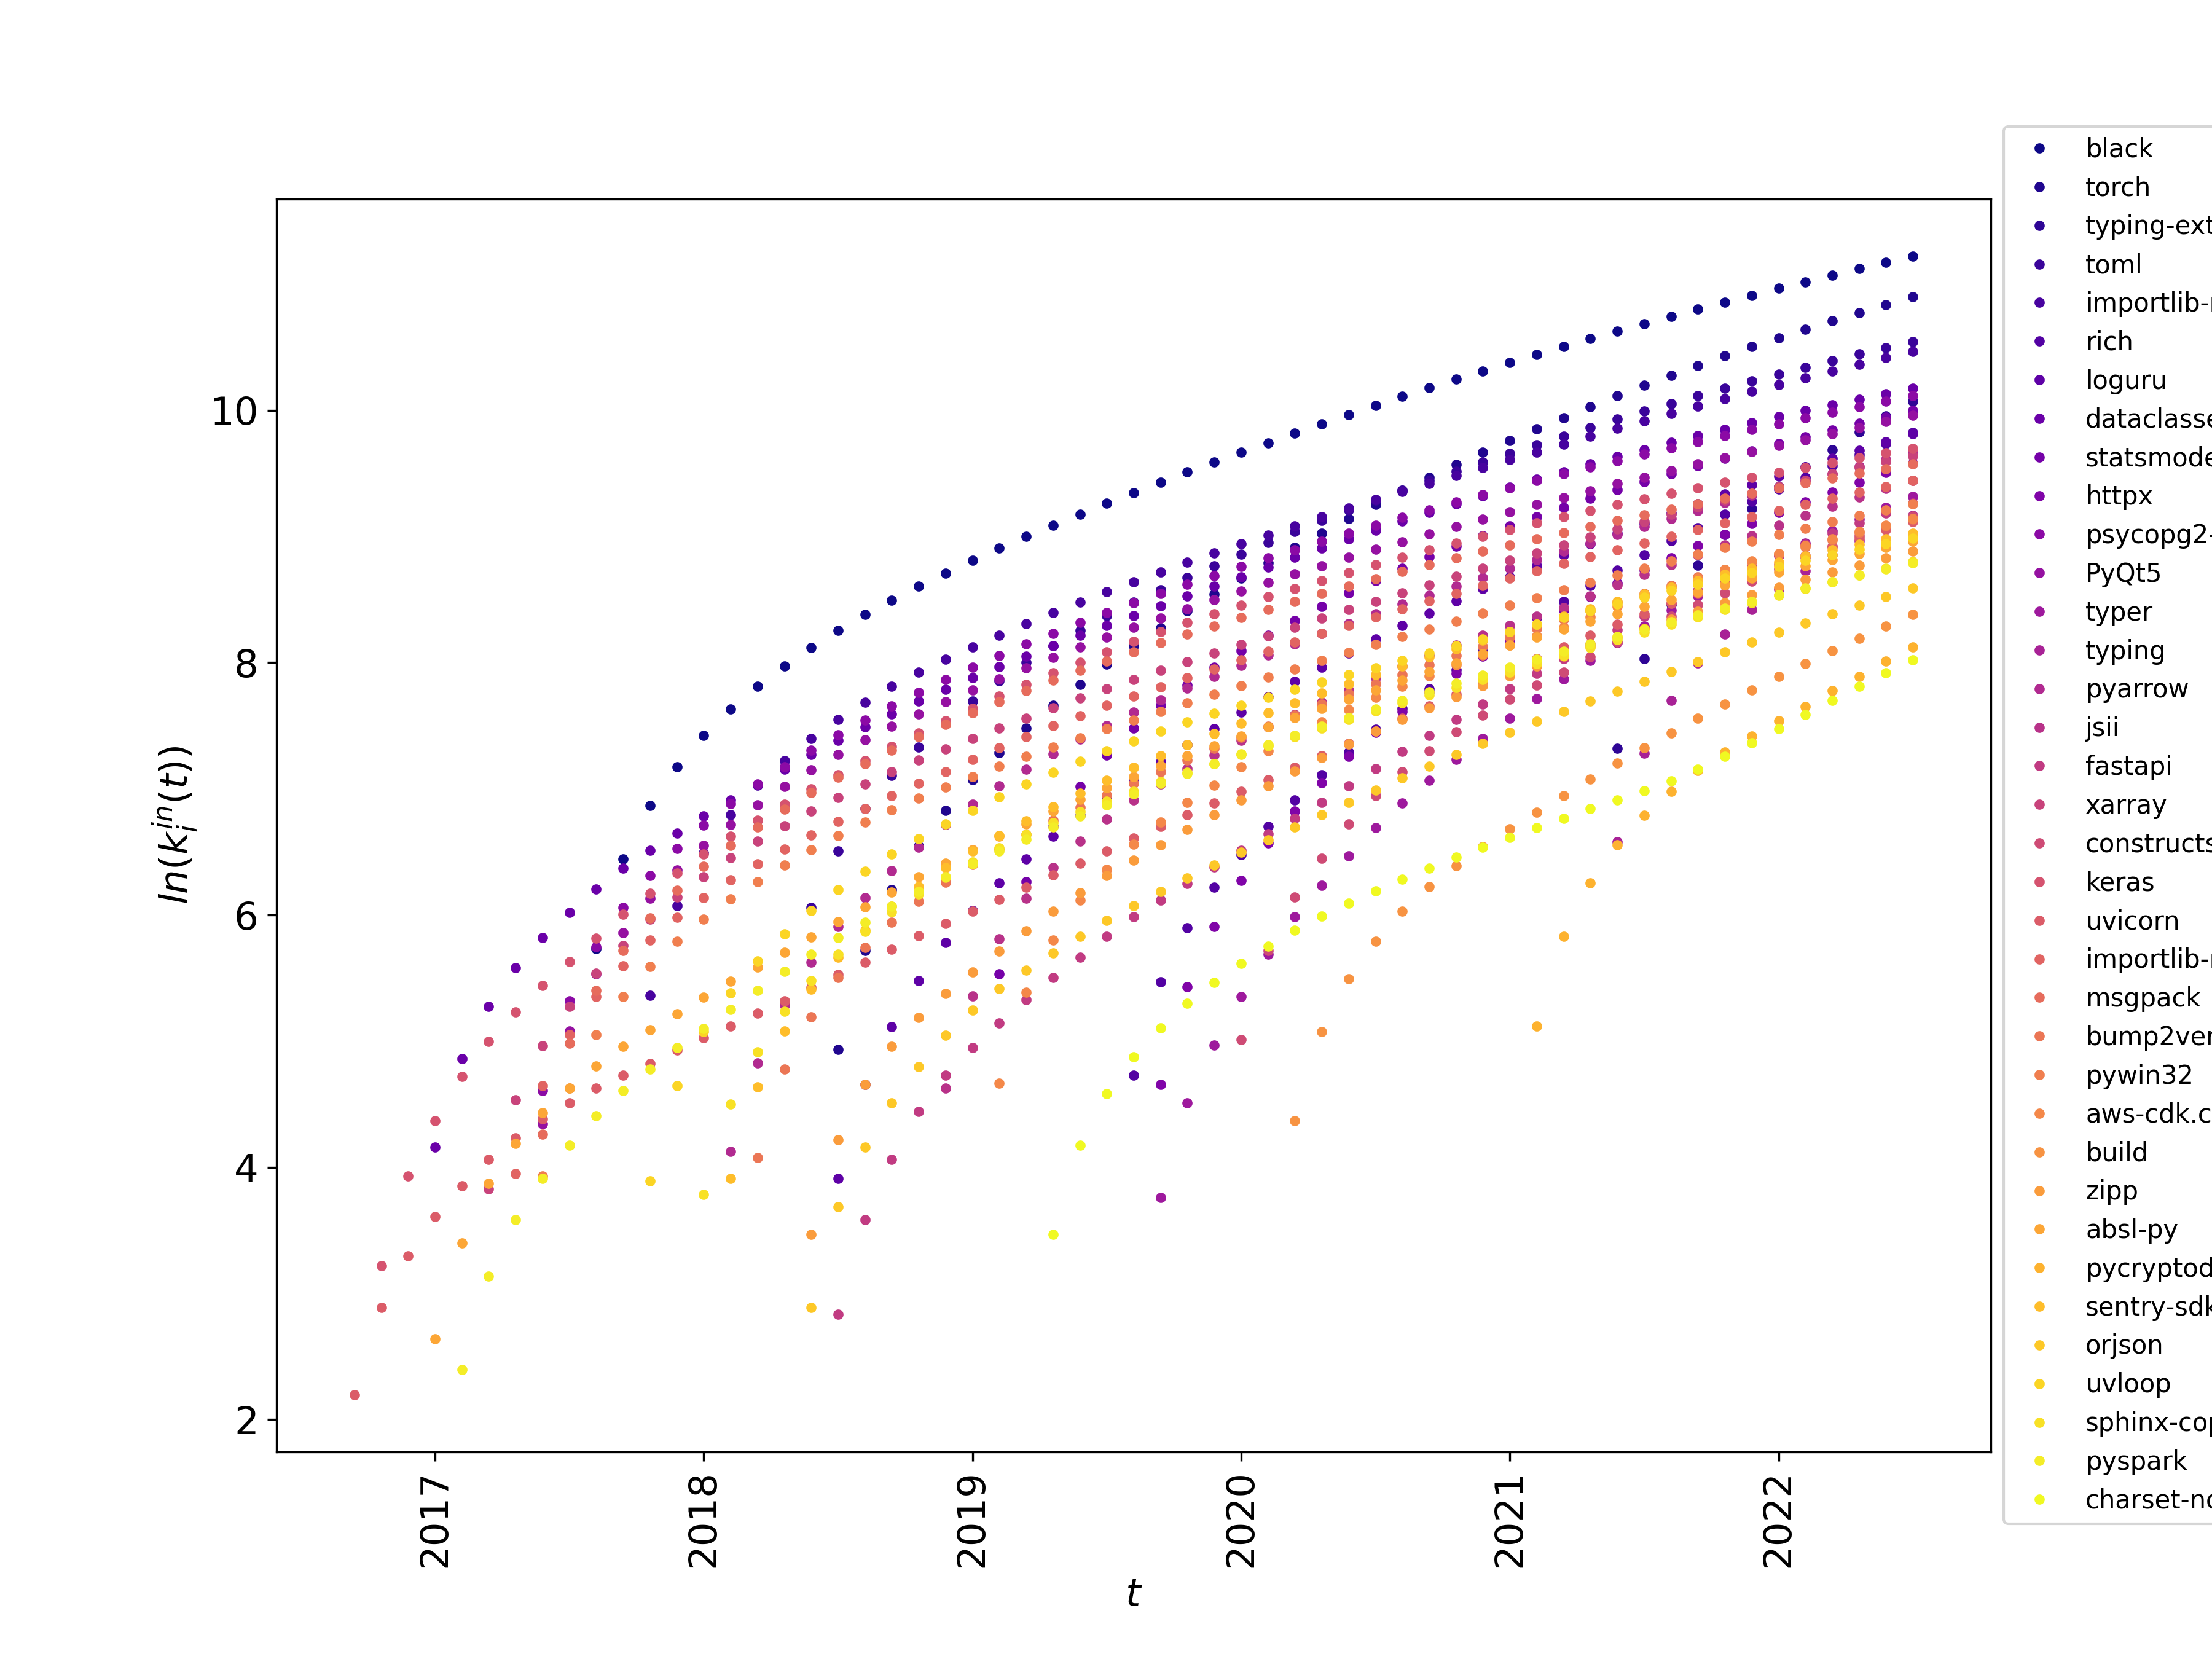
\includegraphics[width=1\textwidth]{../pres/pics/deg_2016_growth.png}
    \caption{Top performing packages based on \textbf{in}-degree growth of
    nodes, released in not before 2016 in a y-log axis}
    \label{fig:findings}
\end{figure}

The final thing now is to visualize the network in Virtual Reality. For this
a layout needed to be created, since the standard spring layout or similar
does not represent the ``pseudo degree hierarchy'' of the network. The main idea is
to visualize the findings in an intuitive way. Based on this a layout
evolving around the degree distribution of the network was made. To make the
explanation comprehensible the reader should think about a bar diagram
representing a power law distribution, the first few bars would be
very big while the last would be very small. The idea is to take all the
nodes in one bar and map them uniformly on a circle starting from the first
bar to the last bar. The disks would be constructed in such a way that they
will visually fit all the nodes inside, i.e. the radius of the disk would
depend on the node size. Have now $n$ circles/disks corresponding to $n$
bars. To make a three dimensional visualization possible, a stacking of these
disks based on a distance function is made. The most visually compelling is
the $\sqrt{\cdot}$ distance function between the disks, so the $n$-th layer
would be $\sqrt{n}$-away from the first layer where the first layer is the
layer with most nodes. The network would look something like the figure above
\begin{figure}[H]
    \centering
    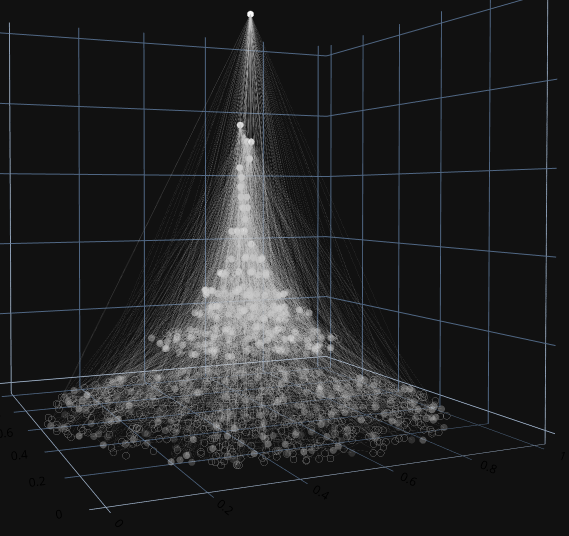
\includegraphics[width=0.8\textwidth]{../pres/pics/plot_sqrt.png}
    \caption{Scale-Free network with layout based on degree distribution}
\end{figure}

In the Virtual-Reality setting, a cut-of of the network is made, removing all
nodes, that have an in-degree below $10$ and painting the predicted nodes in
\ref{fig:findings} red.

\section{Discussion}
In summary, based on an idea, data from the Python Package Index \cite{pypi}
was mapped to a complex network. With the help of release information of each
package, a time evolving network was created. For the sake of dealing with
such graphs a very practical python child class called \texttt{TDiGraph} was
created. It is verified that the network is a scale-free network following a
power-law distribution. Additionally both in the static case and in the
dynamic case of the network, a node degree analysis was made. In the static
case, based on centrality measures. In the dynamic case based on the degree
growth exponent and a release of the node not before 2016. Lastly for the
VR-setting a specific type of layout was constructed based on the networks
degree distribution.

The initial idea for the VR-setting was to really visualize the time
evolution, in a sense  make a ``gif'' in VR. This ``gif'' would start with
a graph $t=T_{2005}$ add nodes and links until $t=T_{2022}$ last step. While
for each step the networks layout needs to be recalculated, because the
setting of the degrees of each time step is different. This kind of structure
would visualize the ``coming up'' of the predicted nodes in \ref{fig:findings}
labeled in red, as they rise through the layers of the network. However this
could not be realized since the unreal engine of the VR-framework did not
allow for node-link removal nor appendage while changing structure.

An additional tweak one could go through is to include user downloads for
each package, this data is also provided by PYPI. The number of user
downloads can be incorporated to construct a weighted graph, which would open
doors to further analysis.

\nocite{barabasi}
\printbibliography
\end{document}
